% !TEX root = deckblatt4.tex
\section{Br\"uckengleichrichter}
\subsection{Aufgabenstellung}
In dieser Aufgabe musste ein Br\"uckengleichrichter aufgebaut werden und Zeit- und Frequenzmessungen durchgef\"uhrt werden. Des weiteren sollte eine Fourierreihe Berechnet und mit den Ergebnissen verglichen werden.

\subsection{Messschaltung}
\begin{figure}[ht!]
  \begin{center}
    \begin{circuitikz}\draw
    (0,0) to[sI] (0,6) to[Do] (7,6) to[R={$R_1$}{$=1M$}](7,0) to[Do] (0,0)
    (2,0) to[short, *-] (2,4) -- (2.5,4) to[Do] (4.5,4) -- (5,4) to[short,-*] (5,6)
    (5,0) to[short, *-] (5,2) -- (4.5,2) to[Do] (2.5,2) -- (1.5,2) to[short, -*] (1.5,6)
    (0,0) node[ground]{};
    \draw[-latex] (8.5,6) -- (7.3,6);
    \draw (9.6,6) node[] {Kanal 1};
    \draw[-latex] (8.5,0) -- (7.3,0);
    \draw (9.6,0) node[] {Kanal 2};
    \draw (3.5,7) node[] {1N4148};
    \end{circuitikz}
  \end{center}
  \caption{Messschaltung}\label{bsp4_circ}
\end{figure}
\noindent
In Abbildung \ref{bsp4_circ} ist der Br\"uckengleichrichter, welcher f\"ur die nachfolgenden Messungen verwendet wird zu sehen. Der Gelichrichter besteht aus vier Dioden (1N4148). Die Ausgangsspannung am Widerstand $R_1$ kann nicht einfach abgegriffen werden da sonst ein Teil der Schaltung \"uber die Masse des Oszilloskops kurgeschlosswern werden w\"urde. Aus diesem Grund wurde mit 2 Kan\"alen gemessen und die Masse der Tastk\"opfe wurde mit der Masse des Funktionsgenerators an einen Punkt geschalten. Anschlie\ss{}end die Differenz mit der "Math"-Funktion des Oszilloskops berrechnet.

\subsection{Messung im Zeitbereich}
\begin{figure}[H]
 \begin{center}
  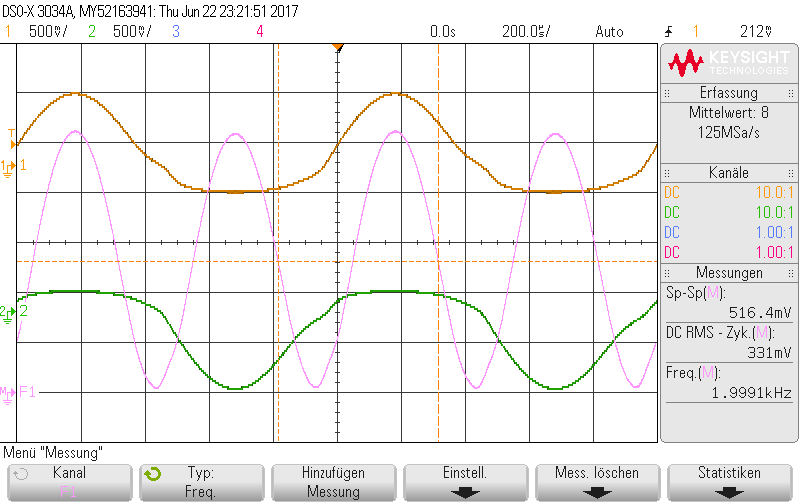
\includegraphics[height=6cm,width=12cm]{OsziBilder/bsp4_sin_time_2Vpp_UeUa.png}
 \end{center}
 \caption{Sinussingal $2V_{pp}$, $1kHz$}\label{bsp4_time2V}
\end{figure}
\noindent

\begin{figure}[H]
 \begin{center}
  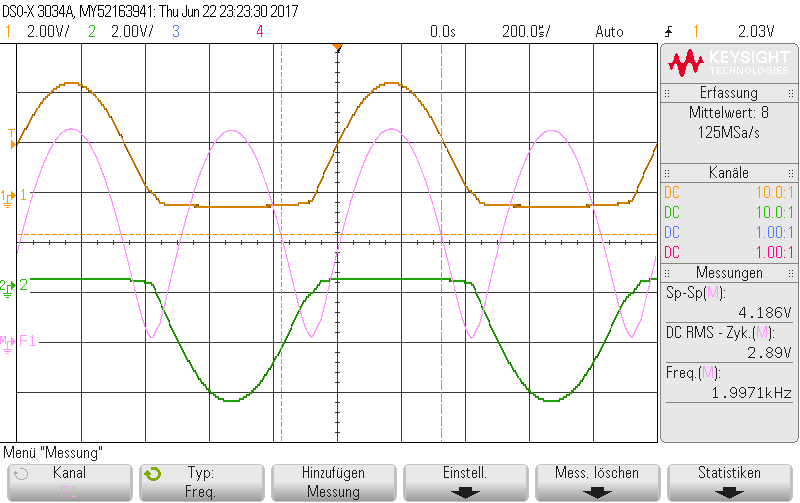
\includegraphics[height=6cm,width=12cm]{OsziBilder/bsp4_time_10Vpp_UeUa.png}
 \end{center}
 \caption{Sinussingal $10V_{pp}$, $1kHz$}\label{bsp4_time10V}
\end{figure}
\noindent
In den beiden Abbildungen \ref{bsp4_time2V} und \ref{bsp4_time10V} sind die Zeitsignale zu sehen. Die Differenz der beiden Kan\"ale ergibt den Gleichgereichteten Sinus, dieser hat die Doppelte Frequnez als das Eingangssignal, jedoch den gleichen Effektiefwert.

\subsection{Fouriereihe}
\begin{center}
  \begin{align*}
    |sin(t)| & \text{ ist eine gerade Funktion} \\ \\
    S(f) &= \frac{a_0}{2} + \sum_{n=1}^{\infty} a_n * cos(nt) \\ \\
    \text{Summensatz S8: } & 2sin(\alpha)cos(\beta) = sin(\alpha-\beta)+sin(\alpha+\beta) \\ \\
    a_0 &= \frac{1}{\pi}\int_0^{2\pi} |sin(t)| dt = \frac{2}{\pi}\int_0^{\pi} sin(t) dt = \frac{4}{\pi} \\ \\
    a_n &= \frac{2}{\pi}\int_0^{\pi} sin(t) * cos (nt) dt \\
    a_n &= \frac{1}{\pi}\int_0^{\pi} sin(t - nt) dt +  \frac{1}{\pi}\int_0^{\pi} sin(t + nt) dt\\
    a_n &= -\frac{1}{\pi} \left[ \frac{cos(\pi(1-n))}{1-n} + \frac{cos(\pi(1+n))}{1+n} \right] \\
    a_n &= -\frac{1}{\pi} \left[ \frac{-(-1)^n-1}{1-n} + \frac{-(-1)^n-1}{1+n} \right] \\
    a_n &= \frac{1}{\pi} \left[ \frac{(-1)^n+1}{1-n} + \frac{-(-1)^n+1}{1+n} \right] \\
    a_n &= \frac{2((-1)^2+1)}{\pi(1-n^2)} \\ \\
    a_n &= \left\{\begin{array}{ll}
            0                     \hspace{2.5cm} \text{f\"ur n ungerade}\\
            \frac{4}{\pi(1-n^2)} \hspace{1.5cm} \text{f\"ur n gerade}
            \end{array}\right.
  \end{align*}
\end{center}

\subsection{FFT}
\begin{figure}[H]
 \begin{center}
  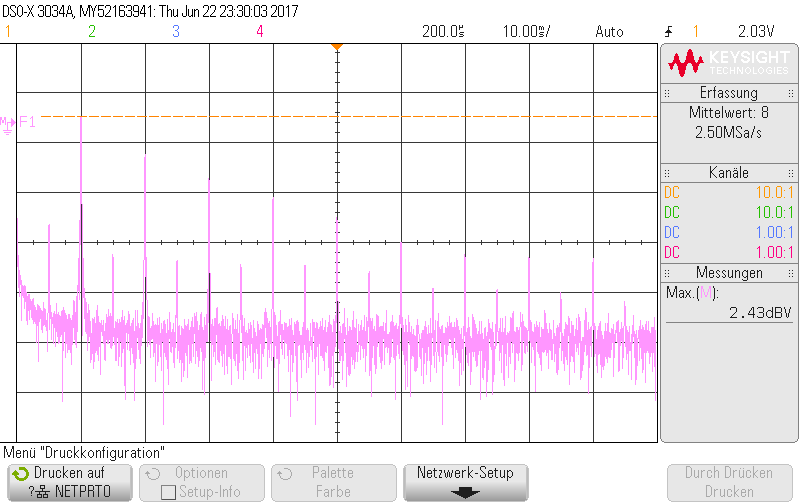
\includegraphics[height=6cm,width=12cm]{OsziBilder/bsp4_sin_fft_10Vpp_dB.png}
 \end{center}
 \caption{Sinussingal $2V_{pp}$, $10kHz$}\label{bsp4_fft}
\end{figure}
\noindent
Genau wie in den Berechnungen ist in dieser Messung zu erkennen, dass jeder zweite Frquenzanteil mit quasi 0 ergibt (ca. $-30dB$) und die Amplituden mit steigender Frequnez rasch kleiner werden.

\begin{figure}[H]
  \begin{center}
    \begin{tabular}{|c|c|} \hline
    $U_0$ & $1,325V$ \\ \hline
    $U_1$ & $231,25mV$ \\ \hline
    $U_2$ & $75mV$ \\ \hline
    $U_3$ & $31,25mV$ \\ \hline
    $U_4$ & $12,2mV$ \\ \hline
    \end{tabular}
  \end{center}
  \caption{Messwerte der f\"unf gr\"o\ss{}ten Spektralen Komponenten}
\end{figure}
\noindent
